\subsection[Mixture models]{Mixture models and model-based clustering}

\begin{frame}{A {parametric} approach}
 Mixture model with $K$ components
	
	$$G = \sum_{k=1}^K \pi_k \delta_{\phi_k}$$
	
	$\delta_{\phi_k}$ is a point mass at ${\phi_k}$.
	
	$G$ is to be understood as a $K$-faceted dice. The  mixture density is:
	$$p(X|\pi,\phi) = \sum_{k=1}^K \pi_k p(x|\phi_k)$$
	
\begin{center}
		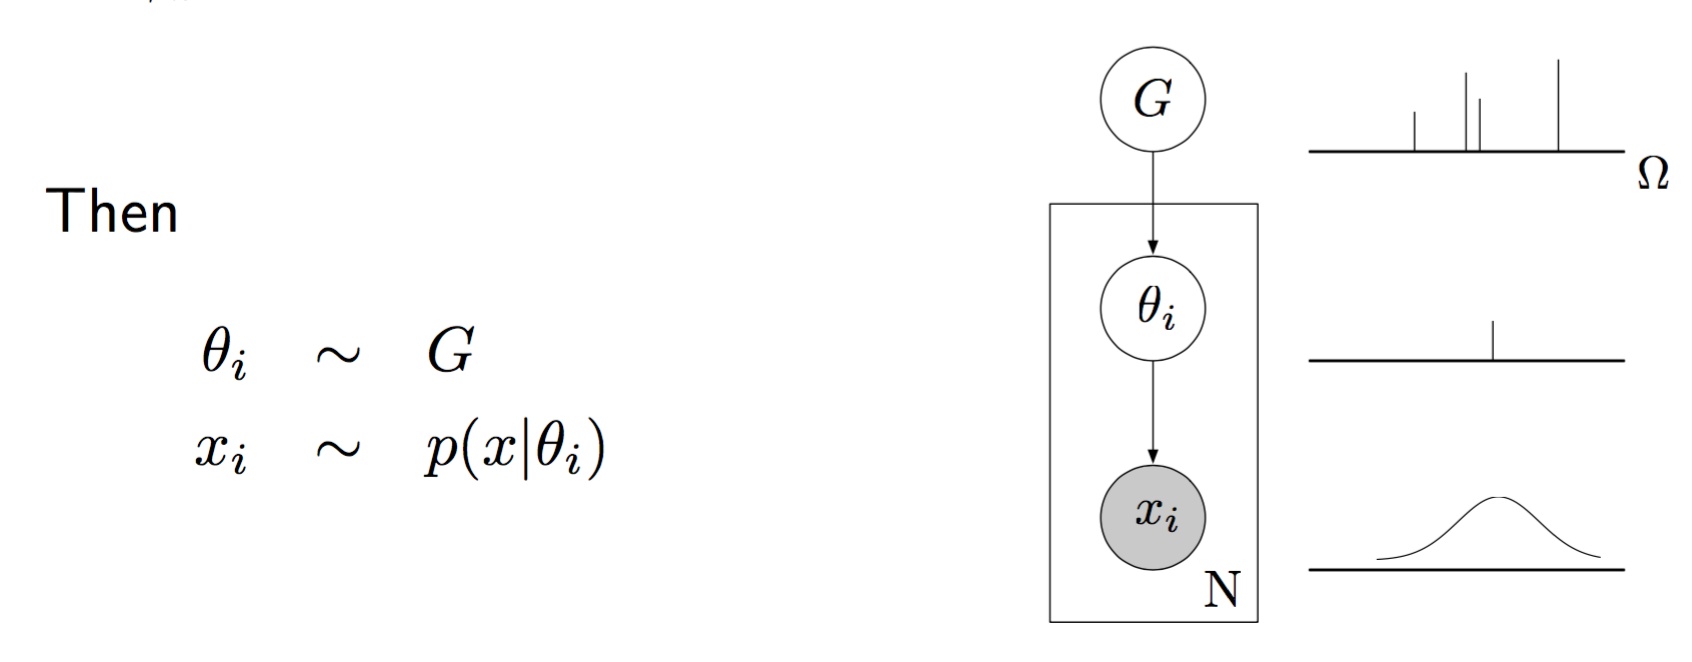
\includegraphics[width=.8\textwidth]{figures_julyan/mixtures/plate_mixture}
\end{center}
\end{frame}



\begin{frame}{A {Bayesian parametric} approach}
	 \alert{Bayesian}   mixture Models with $K$ components
	
We need a distribution over the probability measure (aka dice) $G$, that is a distribution over weights or classes $\pi = (\pi_1,\ldots,\pi_K)$ and over mean and covariance (for 2-dimensional data) $\phi_k = (\mu_k,\Sigma_k)$

\begin{itemize}
	\item $\pi\sim \text{Dirichlet}(\alpha/K, \ldots,\alpha/K)$
	\item $(\mu_k,\Sigma_k)\sim \text{Normal}\times\text{Inverse-Wishart}$
\end{itemize}
This makes $G = \sum_{k=1}^K \pi_k \delta_{\phi_k}$ a random dice

\begin{center}
		\includegraphics[width=.8\textwidth]{figures_julyan/mixtures/plate_bayes_mixture}
\end{center}
\end{frame}

\begin{frame}{Choosing $K$}
There are several options for choosing $K$
\begin{itemize}
	\item Model selection with information criteria: AIC, BIC, or cross-validation, etc
	\item Hierarchical model, with a prior on $K$
	\item Be nonparametric, and let $K$ get large... possibly infinite.
\end{itemize}
	
\end{frame}



\begin{frame}{A {Bayesian nonparametric} approach}
	 \alert{Bayesian nonparametric}   mixture Models
	 
	 We now move to $G$ being an infinite sum $G = \sum_{k=1}^\infty \pi_k \delta_{\phi_k}$ 
	
We need a distribution over this infinite dice $G$, that is exactly what the \alert{Dirichlet process} does. It is parameterized by the precision parameter $\alpha$ and the base measure $G_0$.

\begin{columns}
\column{.45\textwidth}
\begin{itemize}
	\item $\pi = (\pi_1,\pi_2,\ldots)\sim \text{GEM}(\alpha)$
	\item $\phi_k\sim G_0$
\end{itemize}

\column{.45\textwidth}
\begin{center}
		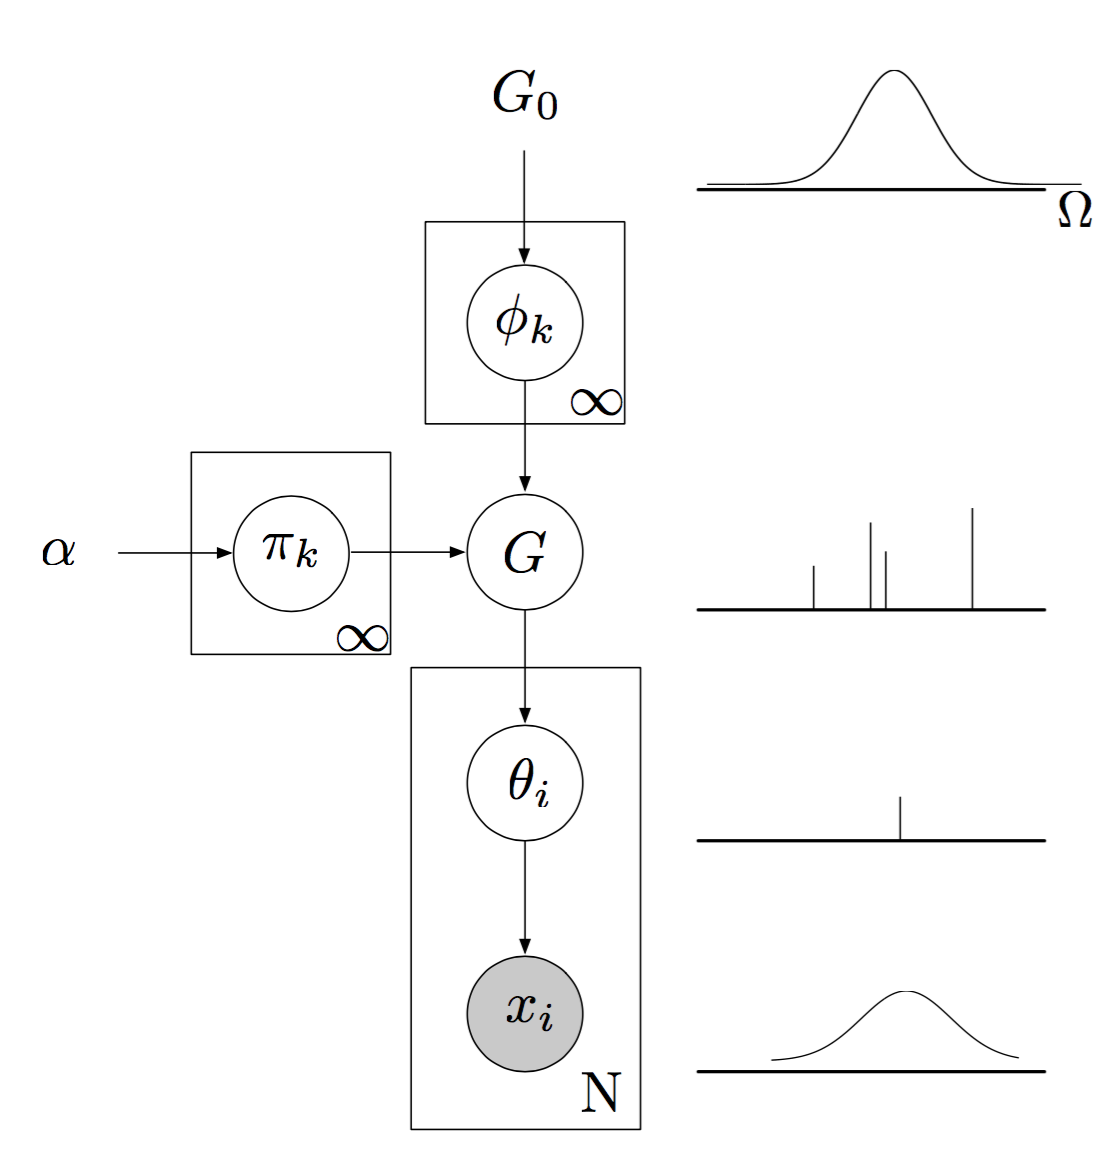
\includegraphics[height=.4\textheight]{figures_julyan/mixtures/plate_SB_mixture}
\end{center}
\end{columns}
\end{frame}



\begin{frame}{Posterior sampling}
Markov chain Monte Carlo (MCMC) methods:
\begin{itemize}
\item \alert{Marginal methods}: marginalizing over the posterior DP $P$, and sampling using the posterior P\'olya urn scheme \citep[easy in conjugate case, see][]{neal2000markov}
\item \alert{Conditional methods}: sampling a finite but sufficient number of parameters
 \citep{ishwaran2001gibbs}. \alert{BNPdensity} R package \citep{arbel2021BNPdensity}.
\end{itemize}
Variational approximations \citep{blei2006variational}
\end{frame}



\begin{frame}[allowframebreaks]{Warning on interpretation of $K_n$}
\begin{columns}

\column{.45\textwidth}

	Consider a simple DP mixture model with
	\begin{itemize}
		\item  Gaussian base measure, 
		\item Gaussian kernel,
		\item where data are sampled  iid from some distribution.
	\end{itemize}
	
Then the \alert{posterior on $K_n$ is inconsistent} \citep{miller2013simple}.
\column{.45\textwidth}
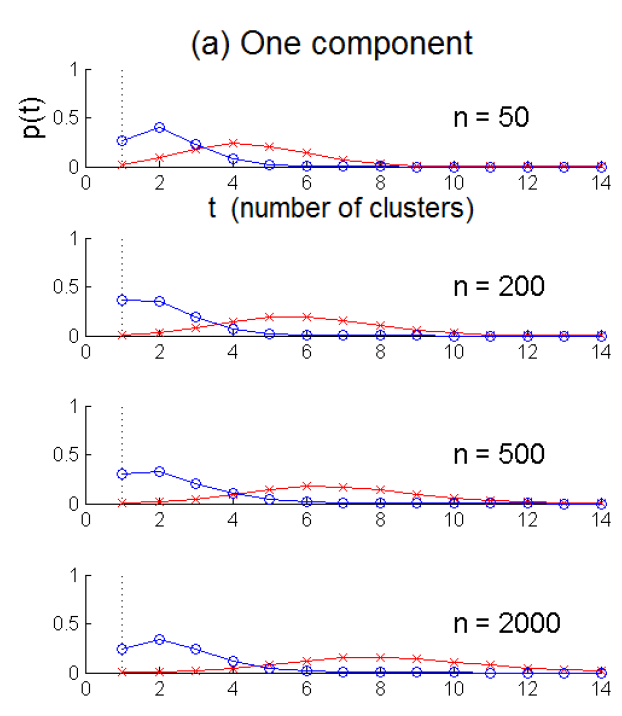
\includegraphics[width=\textwidth]{figures_julyan/mixtures/miller_DP}
\end{columns}
\framebreak

From \citet{miller2013simple} (here $K_n$ is denoted $T_n$):\bigskip

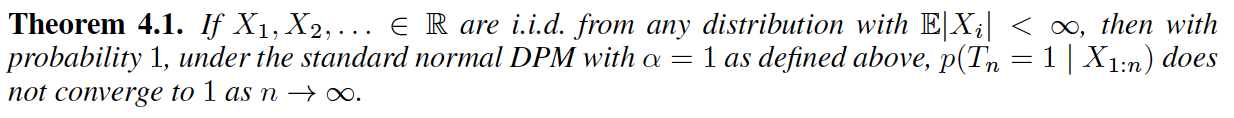
\includegraphics[width=\textwidth]{figures_julyan/mixtures/miller_inconsistency1}\bigskip

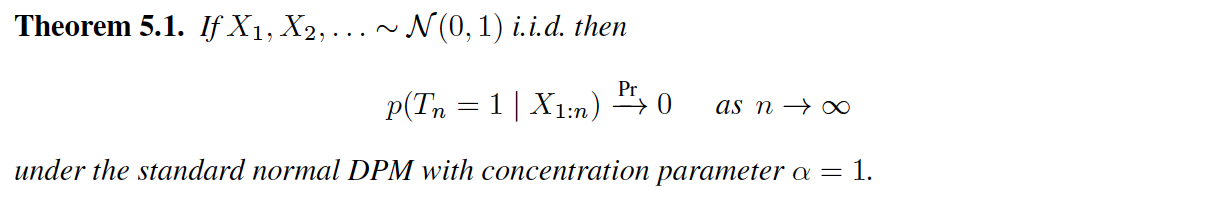
\includegraphics[width=\textwidth]{figures_julyan/mixtures/miller_inconsistency2}\bigskip


But there is some hope...
\end{frame}



\begin{frame}{Bayesian decision theory}
	From decision theory: a Bayes estimator minimizes a posterior expected loss.
	
\begin{equation*}
\hat{a}_L = \arg \inf_{a \in A} \mathbb{E}_{\pi(\theta)}[L_a(\theta)].
\end{equation*}\pause

Examples with Euclidean parameter spaces:
\begin{itemize}
	\item $L^2$, squared loss $\longrightarrow$ posterior mean
	\item $L^1$, absolute loss $\longrightarrow$ posterior median
	\item $0-1$ loss  $\longrightarrow$ mode a posteriori (MAP)
\end{itemize}
\end{frame}

\begin{frame}{Deriving an optimal clustering}

The posterior expected loss of clustering $c'$, denoted by $L(c')$, is obtained by \alert{averaging the loss with respect to posterior weight}
$$L(c') = \sum_{c\in\Ac_n} L(c,c')p(c|\bx),$$
and the decision is taken by choosing the best

\begin{equation*}
\hat c = \arg \min_{c' \in \Ac_n} \sum_{c\in\Ac_n} L(c,c')p(c|\bx)
\end{equation*}\pause
Several losses have been considered:
	\begin{itemize}
		\item 0-1 loss \citep{rajkowski2019analysis},
		\item Binder loss \citep{dahl2006model},
		\item Variation of information \citep{wade2018bayesian}.
	\end{itemize}
\end{frame}

\begin{frame}{Simplest loss: $L_{0-1}$}

\begin{align*}
	L_{0-1}(c') = \sum_{c\in\Ac_n} L_{0-1}(c,c')p(c|\bx) &= \sum_{c\in\Ac_n,\,c\neq c'} p(c|\bx),\\
	& = 1 - p(c'|\bx)\pause
\end{align*}
which is to say that the expected loss of $c'$ is \alert{all the posterior mass except that of $c'$.} So that it is easily minimized at the value $c'$ which has \alert{maximum} posterior weight:
$$\hat c =  \arg \min_{c' \in \Ac_n} L_{0-1}(c') =   \arg \max_{c' \in \Ac_n} p(c'|\bx):= MAP.$$\pause

Negative results by \citet{rajkowski2019analysis} show that the \alert{mode a posteriori (MAP) is inconsistent}.
	
\end{frame}

\begin{frame}{Variation of information}
\alert{Variation of information} (VI) by \citet{meila2007comparing} for cluster comparison. From information theory, compares information in two clusterings with information shared between the two clusterings:
\begin{align*}
&\VI(\bc,\widehat{\bc})=\En(\bc)+\En(\widehat{\bc})-2\I(\bc,\widehat{\bc})
\end{align*}
\end{frame}


\begin{frame}{Variation of information}
\citet{wade2018bayesian} 
compare Binder and VI:\bigskip

\begin{center}
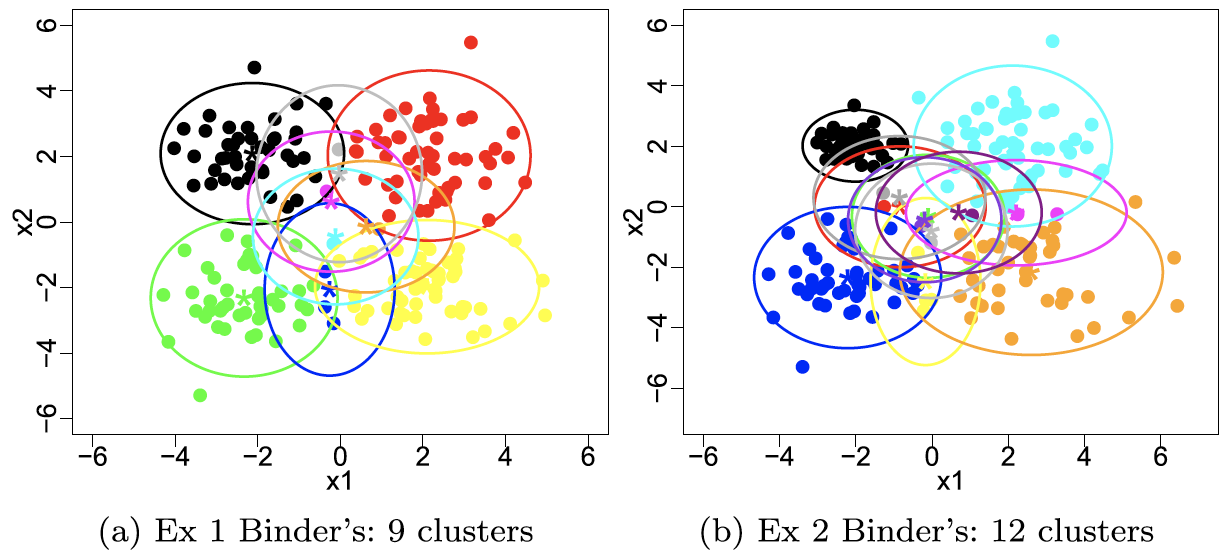
\includegraphics[width=.7\textwidth]{figures_julyan/mixtures/wade_example_binder}
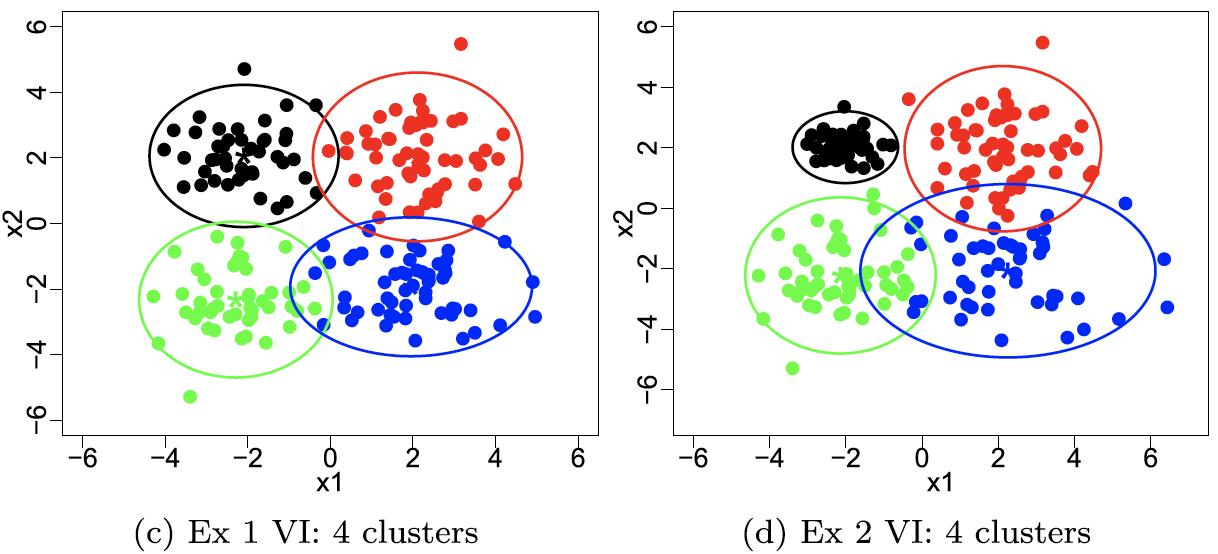
\includegraphics[width=.7\textwidth]{figures_julyan/mixtures/wade_example_VI}	
\end{center}
\end{frame}


\begin{frame}{Variation of information}
\citet{wade2018bayesian} 
also provide \alert{credible balls} around the estimated clustering, based on Hasse diagram:\bigskip

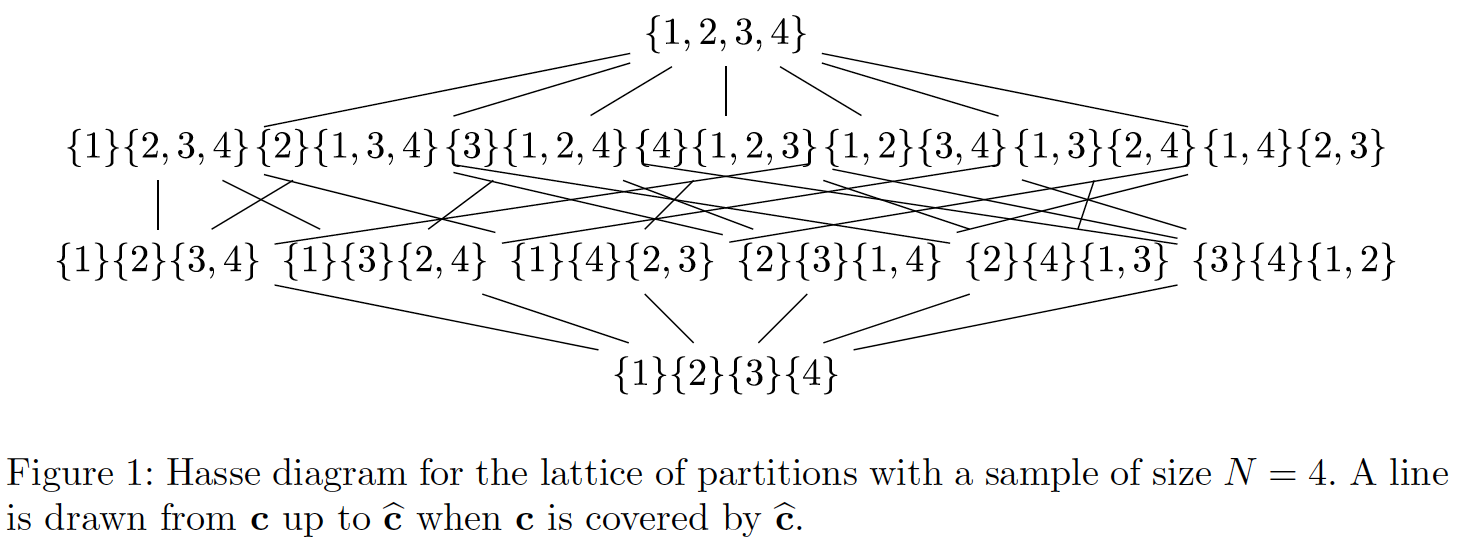
\includegraphics[width=\textwidth]{figures_julyan/mixtures/hasse_diagram}
\end{frame}